\documentclass[10pt]{beamer}
	\useoutertheme{infolines}
	\usetheme{metropolis}       % Use metropolis theme
	\metroset{progressbar=head, titleformat=smallcaps, numbering=fraction, block=fill}

\pdfstringdefDisableCommands{\let\uppercase\relax}

\setbeamertemplate{section in toc}[sections numbered]

\usepackage{color, colortbl}    % Use table colors
	\definecolor{Gray}{gray}{0.8}

\usepackage{caption}            % Use caption scriptsize
	\captionsetup{font=scriptsize,labelfont=scriptsize}

\usepackage[english]{babel}
\usepackage{inputenc}
\usepackage{fontenc}
\usepackage{xspace}
\usepackage{libertine}
\usepackage{multirow}
\usepackage{amssymb}
\usepackage{amsmath}
\usepackage{enumerate}
\usepackage{pgfplots}
\usepackage{natbib}
\usepackage{subcaption}

\newcommand{\themename}{\textbf{\textsc{metropolis}}\xspace}

\pdfstringdefDisableCommands{\let\uppercase\relax}

% ----------------------------------------------------------------- %

\title{Estimation and Validation of \\ Agent-based Computational Economic Models}
\author{Guerini Mattia}
\institute{Université Côte d'Azur - GREDEG}
\date{\today}

% ----------------------------------------------------------------- %

\begin{document}


\begin{frame}
	\begin{figure}[htbp] \centering \hfill 
		
\includegraphics[scale=.10]{logo/gredeg.png} ~
		
\includegraphics[scale=.15]{logo/acepol.png} %~
		% \includegraphics[scale=.04]{logo/mca.png}
	\end{figure}

	\vspace{-2cm}
	\maketitle
\end{frame}


\begin{frame}[c]\frametitle{Table of Contents}
	\tableofcontents[hideallsubsections]
\end{frame}


% ----------------------------------------------------------------- %


% intro ----------------------------------------------------------- %
% \section{Critiques to ACE models}
% \label{sec:ace_critiques}


% \subsection{Absence of standard characteristics}


% \begin{frame}[c]\frametitle{ACE models lack of standard characteristics}
	
% 	\alert{\textbf{Missing characteristics in an ACE model}}
% 	\begin{itemize}
% 		\item agents with an optimizing behaviour;
% 		\item understandable transmission mechanisms;
% 		\item clarity in the causal relationships.
% 	\end{itemize} \bigskip
	
% 	Are critiques based on these arguments well-founded? 
% 	\begin{itemize}
% 		\item not in general \citep{gigerenzer2009heuristicus};
% 		\item partially \citep{meisser2017code};
% 		\item no \citep{moneta2005causality}.
% 	\end{itemize}
% \end{frame}	


% \begin{frame}[c]\frametitle{A discussion on the \emph{primitives}}
% 	The departure from the axiomatic approach and the optimizing behaviour casts doubts on ACE models from a model-consistency perspective. ACE abandons the \emph{primitives} of traditional economic models. \bigskip

% 	But once the axioms are abandoned, what psychological motives determine agents' choices? \bigskip

% 	\alert{\textbf{Heuristics}}
% 	\\ Cognitive processes that ignore some of the information. Still, they can be efficient in uncertain and complex environments \citep{gigerenzer2009heuristicus}. \bigskip

% 	In ACE models, heuristics are the \emph{psychological primitives}. But they suffer of the wilderness of bounded rationality problem (i.e. which heuristic to choose?)
% \end{frame}


% \begin{frame}[c]\frametitle{Different grounds between causality and explanation}
% 	Transmission mechanisms are often very clear to the modeller of an ACE model, but they are difficult to be explained as emergent properties of a complex system \citep[see][]{anderson1972science}. \bigskip

% 	The causal relations therefore -- in the realistic interpretation of the word -- exist only at the micro level and are inherited from the \emph{primitive} behavioural rules. \bigskip

% 	The economic transmission mechanisms are instead embedded in the computer programme, which is nothing but a sequence of explicable orders performed by a machine \citep{meisser2017code,valente2017knowledge}. \bigskip

% 	\alert{\textbf{More is different}}
% 	\\ But even knowing the real micro-level causality, most of the time one is interested in the relation between different emergent properties. These relations can eventually be interpreted only under a different notion of causality -- reductionist approach, \citep[see][]{moneta2005causality}.
% \end{frame}


% \begin{frame}[c]\frametitle{The inductive nature of ACE models}
% 	\alert{\textbf{Methodological distinction}}
% 	\begin{itemize}
% 		\item \emph{traditional models} follow the deductive method: from the axioms and the optimization problem, result are deduced under the form of theorems and proofs; 
% 		\item \emph{ACE models} follow the inductive method: the behavioural rules induce the generation of aggregate emergent properties, to which an economic argumentation can only be attached by means of statistical or anecdotal evidence.
% 	\end{itemize} \bigskip
	
% 	ACE models do not display a homotetic behaviour between micro- and macro- dynamics. This creates a difficulty in explaining the results from an Agent-Based Model (ABM). \bigskip

% 	A reductionist approach to causality might decrease this communicational difficulty.
% \end{frame}


% \subsection{Presence of non-standard characteristics}


% \begin{frame}[c]\frametitle{ACE models embed non-standard characteristics}
% 	\alert{\textbf{Typical characteristics in an ACE model}}
% 	\begin{itemize}
% 		\item \emph{ad-hoc} behavioural assumptions;
% 		\item large numbers of free parameters -- somehow too many;
% 		\item simulations with some incredible values.
% 	\end{itemize} \bigskip

% 	Are critiques based on these arguments well-founded? 
% 	\begin{itemize}
% 		\item yes (but solvable);
% 		\item yes (but solvable);
% 		\item not in general \citep{marks2013validation}.
% 	\end{itemize}
% \end{frame}


% \begin{frame}[c]\frametitle{An expedition in the wilderness of bounded rationality}
    
%     \alert{\textbf{How to select among all the possible heuristics?}}
%     \begin{quote}
%     	There is only one way to be rational. But there are infinitely many different ways to be irrational. \\ \hfill \citet{hommes2013book}
%     \end{quote}

%     Developing sub-literatures in the behavioural economics domain:
%     \begin{itemize}
%     	\item empirical micro evidence \citep{dosi2004simon};
%     	\item management science approach \citep{dawid2012approach};
%     	\item experimental economics \citep{hommes2013book}.
%     \end{itemize} \bigskip

%     \citet{dawid2018handbook} have recently classified the behavioural rules adopted in ABM under a bunch of common general principles.
% \end{frame}


\begin{frame}[c]\frametitle{Critique to ACE models}
	\begin{itemize}
		\item \emph{ad-hoc} behavioural assumptions;
		\item large numbers of free parameters -- somehow too many;
		\item simulations with some incredible values.
	\end{itemize} \bigskip
	
	The last two are \alert{\textbf{technical and valuable critiques}} (acknowledged also by AB modellers) \bigskip

	However:
	\begin{itemize}
		\item many parameters in ABM are \emph{deep} and can therefore be estimated; % they are constitutive of the behavioural rules
		\item there exist tools to estimate ACE models; % the topic of this short course
		\item ABM are not the unique ones facing these problems \citep{fagiolo2017redux}. % see DSGE large models at central banks
	\end{itemize} \bigskip

	% About the incredibility of simulation values, one shall always distinguish between:
	% \begin{itemize}
	% 	\item demonstration models;
	% 	\item descriptive models.
	% \end{itemize}
\end{frame}


% definitions ----------------------------------------------------- %
\section{Glossary and definitions}


\begin{frame}[c]\frametitle{Classes of models}
	\alert{\textbf{Demonstration models}} 
	\\ Existence proofs for phenomena of interest. They are also called \emph{exploration models} because of their primary objective is that of unveiling the presence of some possible mechanism at work. \bigskip

	\alert{\textbf{Descriptive models}} 
	\\ Attempt to track dynamic historical phenomena. Their primary aims are that of qualitatively or/and quantitatively mimic the dynamics of some real phenomenon and to explain it by means of the economic forces embedded in the model.

	Both types of models require verification; only the second class requires validation (and credible values).
\end{frame}


\begin{frame}[c]\frametitle{Stylized facts}
	\alert{\textbf{Stylized fact (SF)}} 
	\\ An empirical/statistical regularity. \bigskip

	\begin{quote}
		Facts as recorded by statisticians are always subject to numerous snags and qualifications, and for that reason are incapable of being summarized. \\ \hfill \citet{kaldor1957styfacts}
	\end{quote}

	SF can be characterized by different degrees of:
	\begin{itemize}
		\item robustness;
		\item generality;
		\item easiness of generation.
	\end{itemize} \bigskip

	Replication of SF does not mean the model is a descriptive one, but a descriptive model shall replicate (at least some) SF \citep{brock1999scaling,buchanan2012stylizedfact,fagiolo2019validation,guerini2017validation}.
\end{frame}


\begin{frame}[c]\frametitle{Parameters' space exploration}
    \alert{\textbf{Parameters' space exploration} (\emph{sensitivity analysis})}
    \\ Replies to the question: \emph{How the model's outcome is affected by a variations in one parameter?} \\ Is a sort of model elasticity w.r.t. a change in the parameters \citep{salle2014kriging}. \smallskip

    Trade-off:
    \begin{itemize}
    	\item \textbf{robust model}: ideally you don't want that all the results change as soon as you change one parameter (unless that's the scope of the parameter within the model);
    	\item \textbf{tautological model}: ideally you don't want a model whose outcome is equivalent for all the values of a parameter (in that case it is likely that the parameter does not play any role and can be dropped).\footnote{Under the assumption that a parsimonious model is better than an overly complicated one.}
    \end{itemize}
\end{frame}


\begin{frame}[c]\frametitle{Model stationarity and model ergodicity}
	\alert{\textbf{Model Stationarity}} 
	\\ A model is said to be stationary if, after a certain period $T_{s}$, the main variable(s) under scrutiny converges to a time-invariant distribution; \bigskip 

	\alert{\textbf{Model Ergodicity}} 
	\\ A model is said to be ergodic if, after a certain period $T_{s}$, the main variable(s) under scrutiny converges to a time-invariant distribution and the distribution is the same for all the Monte Carlo simulations. \bigskip
\end{frame}


\begin{frame}[c]\frametitle{Verification and validation (V\&V)}
	\alert{\textbf{Model Verification}} 
	\\ Replies to the question \emph{are we building the model right?} \\ It is a formal requirement on the efficacy of the code to be correctly representing the conceptual model under study (i.e. the economic forces at stake) \citep{yilmaz2006verification,naylor1967verification}. Any model should satisfy this requirement. \bigskip % reproducibility and code sharing is one possibility for enhancing the verification of a model

	\alert{\textbf{Model Validation}} 
	\\ Replies to the question \emph{are we building the right model?} \\ It consists of measuring and evaluating the extent to which the model that we have designed is a good representation of the reality \citep{marks2013validation}. Not all models are built to be validated. \bigskip

	%\textbf{Note}: there is both a philosophical and a methodological difference between the two.
\end{frame}


\begin{frame}[c]\frametitle{Calibration and estimation}
	\alert{\textbf{Model Calibration}} 
	\\ Finding the parameter values that allow the model to resemble as close as possible some properties of the data (ex-ante, it does not pretend that the model is a representation of the true DGP). \bigskip

	\alert{\textbf{Model Estimation}} 
	\\ Finding the parameters values that are most likely to have generated the observed empirical data series (ex-ante, it assumes that the model is the true representation of the DGP). \bigskip

	\textbf{Note}: there is only a philosophical difference between the two. Methodologically, they converge to overlapping exercises.\footnote{In what follows I will use the two concepts as identical.}
\end{frame}

% calibration/estimation -------------------------------------------- %
\section{Estimation of ACE models}
\label{sec:estimation_general}

% \begin{frame}[c]\frametitle{The calibration problem}
% 	\begin{quote}
% 	Calibration is the strategy for finding numerical values for the parameters of artificial economic worlds. \\ \hfill \citet{cooley1997calibrated}.
% 	\end{quote} \bigskip

% 	\begin{quote}
% 	A model is calibrated when its parameters are quantified from casual empiricism or unrelated econometric studies or are chosen to guarantee that the model mimics some particular feature of the historical data.  \\ \hfill \citet{hoover1995artifacts}.
% 	\end{quote}
% \end{frame}


\begin{frame}[c]\frametitle{Indirect inference}
	A simulation-based method for estimating the parameters of economic models where the likelihood function is intractable \citep{gourieroux1993indirect}. \bigskip 

	\alert{\textbf{General procedure}}
	\begin{itemize}
		\item simulate data from the economic model for different values of its parameters;
		\item use an \emph{auxiliary model} to form a criterion function;
		\item determine the parametrization at which the model and the observed data look most similar.
	\end{itemize} \bigskip
	
	The objective is that of choosing the parameter vector such that the observed data and the simulated data look most similar from the point of view of the chosen auxiliary model.
\end{frame}


\begin{frame}[c]\frametitle{A formal description}
	\alert{\textbf{The ACE model}}
	\\ Let:
	\begin{equation}
		y_{t} = \mathcal{G}(y_{t-1}, x_{t}, u_{t}; \theta), \quad t = 1,\dots,T, \quad y_{0} = \hat{y}_{0}, \quad u_{t} \sim iid
	\end{equation}
	describe the DGP (i.e. our ACE model). $\mathcal{G}$ can be interpreted as a probability density function for $y_{t}$ conditional on $y_{t-1}$ and $x_{t}$, depending also on the $k$-dimensional parameter vector $\theta$. \medskip

	An econometrician would approach the problem by using the observed data to estimate the k-dimensional parameter vector $\hat{\theta}$. \medskip

	Standard inference tools -- e.g. Maximum Likelihood Estimation (MLE) -- require that $\mathcal{G}$ has an analytical closed form such that a likelihood function can be derived and the optimal $\theta^{*}$ can be estimated. \medskip 
	
	Indirect inference helps when $\mathcal{G}$ is too complex to have a closed form. That's why it is particularly suited for ABM, where $\mathcal{G}$ typically represents a high-dimensional and possibly non-linear model.
\end{frame}


\begin{frame}[c]\frametitle{Indirect inference}
    \alert{\textbf{The auxiliary model (on actual data)}}
	\\ Let:
	\begin{equation}
		\mathcal{F}(y_{t} | y_{t-1}, x_{t}; \beta)
	\end{equation}
	be an auxiliary model (sufficiently simple) depending on the p-dimensional parameter vector $\beta$ (with $p \geq k$) which can also be incorrectly specified. \medskip %\footnote{It is misspecified if it does not correspond to the conditional probability given by $\mathcal{G}$.} \bigskip

	The parameters $\hat{\beta}$ can be estimated using the actual data as:
	\begin{equation}
		\hat{\beta} = \underset{\beta}{argmax} \sum_{t=1}^{T} log \mathcal{F}(y_{t} | y_{t-1}, x_{t}; \beta)
	\end{equation}
\end{frame}


\begin{frame}[c]\frametitle{Indirect inference}
    \textbf{The auxiliary model (on simulated data)}
    \\ The parameters $\beta$ of the auxiliary model $\mathcal{F}$ can also be estimated over the simulated data. \bigskip

    \textbf{Procedure}:
    \begin{itemize}
    	\item draw the disturbances $u_{m,t}$, with $m = 1, \dots, M$ and $t = 1, \dots, T$ from a defined probability distribution;
    	\item pick a parameter vector $\theta$ and iterate the model $\mathcal{G}(\theta)$ to generate a random sequence of the variables of interest $\tilde{y}_{m,t}(\theta)$;
    	\item maximize the average of the log-likelihood across the $M$ simulations to obtain:
    	\begin{equation}
    		\tilde{\beta}(\theta) = \underset{\beta}{argmax} \sum_{m=1}^{M} \sum_{t=1}^{T} log \mathcal{F}(\tilde{y}_{m,t}(\theta) | \tilde{y}_{m,t-1}(\theta), x_{t}; \beta)~;
    	\end{equation}
    	\item select the values $\theta$ that minimizes the distance between $\hat{\beta}$ and $\tilde{\beta}(\theta)$.
    \end{itemize}
\end{frame}


\begin{frame}[c]\frametitle{Similarity measure}
    When using indirect inference, it is necessary to choose a metric for measuring the distance between the parameters of the auxiliary model estimated respectively with real and simulated data. \bigskip

    {}
    There are three possibilities corresponding to the classical trinity of testing: 
	\begin{align*}
		\hat{\theta}^{WA} & = \underset{\theta}{argmin} \left[ \left(\hat{\beta} - \tilde{\beta}(\theta)\right)' W \left(\hat{\beta} - \tilde{\beta}(\theta) \right) \right] \\ \vspace{.2cm}
		\hat{\theta}^{LR} & = \underset{\theta}{argmin} \left[ \sum_{t=1}^{T} log \mathcal{F}(y_{t} | y_{t-1}, x_{t}; \hat{\beta}) -  \sum_{t=1}^{T} log \mathcal{F}(y_{t} | y_{t-1}, x_{t}; \tilde{\beta}(\theta))\right] \\ \vspace{.2cm}
		\hat{\theta}^{LM} & = \underset{\theta}{argmin} \left[ S(\theta)' V S(\theta) \right], \qquad S(\theta) = \sum_m \sum_t \frac{\partial}{\partial \beta} \left[ log \mathcal{F} \left( \tilde{y}_{t}^{m} (\theta) | \tilde{y}_{t-1}^{m}, x_{t}; \hat{\beta} \right) \right]
	\end{align*}
	where $W$ and $V$ are two positive-definite weighting matrices.
\end{frame}


% \begin{frame}[c]\frametitle{Choosing the distance}
%     If the auxiliary model $\mathcal{F}$ is just-identified, the three deliver the same estimate $\beta$ and are also identical to the (infeasible, due to the complexity of $\mathcal{G}$) MLE. \bigskip

%     When the auxiliary model is over-identified, the minimized values of the three metrics are greater than zero and the estimated $\hat{\theta}$ might also differ between them. \bigskip 

%     The minimized values can therefore be used to test the hypothesis that the economic model is correctly specified: sufficiently large minimized values constitute evidence against the auxiliary model.
% \end{frame}


\begin{frame}[c]\frametitle{Pros and cons for ACE applications}
    \alert{\textbf{Advantages}} 
    \begin{itemize}
    	\item relies on estimators with well known statistical properties;
    	\item even if the auxiliary model is incorrect, the estimation can be correct;
    	\item it is the natural extension of a classical econometric problem.
    \end{itemize}

    \alert{\textbf{Drawbacks}} 
    \begin{itemize}
    	\item the estimation error increases with the dimensionality of the problem;
    	\item requires the simulation of the true model over a large set of parameter values and with many Monte Carlo runs (might be computationally heavy);
    	\item results on the optimal choice of $\theta$ might depend upon:
    	\begin{itemize}
    	 	\item the chosen objective variables;
    	 	\item the chosen distance measure;
    	 	\item the number of Monte Carlo replications.
    	\end{itemize} 
    \end{itemize}
\end{frame}


\begin{frame}[c]\frametitle{Particular cases}
	
	The \alert{\textbf{Simulated Minimum Distance}} \citep[SMD - ][]{hsiao1989smd} and the \alert{\textbf{Method of Simulated Moments}} \citep[MSM - ][]{mcfadden1989msm} can be seen as special cases of the indirect inference, where the auxiliary models on which the estimation exercise is based are:
	\begin{itemize}
	 	\item one or few parameters estimated from a simple econometric model involving the variables of interest (e.g. the Pareto-tail parameter of the size distribution of firms);
	 	\item one or few low order moments concerning the variables of interest (e.g. average growth rate of GDP).
	 \end{itemize}
\end{frame}


% estimation in low-dimensions ------------
\section{Estimation of small-scale ABM}
\label{sec:smallscale_abm}


\subsection{Gilli and Winker (2001)}


\begin{frame}[c]\frametitle{\citet{gilli2001estimation}}
	\citet{gilli2001estimation} have been the pioneers in this field of research by applying the indirect inference method to ACE models. \bigskip

	\alert{\textbf{Main features}}
	\begin{itemize}
		\item Simple ABM of the foreign exchange market \citep[the][\emph{ant model}]{kirman1991epidemics};
		\item Dataset on the daily log-returns of the DM/US\$ exchange rate;
		\item Two key data properties to be matched:
		\begin{itemize}
			\item the excess kurtosis at daily frequency $k_{d}$;
			\item the volatility clustering parameter $\alpha_{1}$.
		\end{itemize}
	\end{itemize}
\end{frame}


\begin{frame}[c]\frametitle{The description of the model}
    Two types of agents: 
    \begin{itemize}
    	\item fundamentalist: $E^{f}[\Delta S_{t+1}] = \nu (\bar{S} - S_{t})$;
    	\item chartist: $E^{c}[\Delta S_{t+1}] = S_{t} - S_{t-1}$.
    \end{itemize} 

    An agent might change rule due to:
    \begin{itemize}
    	\item random mutation, with a fixed probability $\varepsilon$;
    	\item conviction, with a fixed probability $\delta$ and after having interacted with a second individual.
    \end{itemize}
    
    The market price is determined as:
    \begin{equation}
    	E^{m}[\Delta S_{t+1}] = w_{t} E^{f}[\Delta S_{t+1}] + (1- w_{t}) E^{c}[\Delta S_{t+1}].
    \end{equation}
\end{frame}


\begin{frame}[c]\frametitle{Simulated Minimum Distance}
	The indirect inference procedure for the estimation of the two parameters $(\varepsilon, \delta)$ solves the following minimization problem:
	\begin{equation}
		f = |\bar{\hat{k}}_{d} - k_{d}| + |\bar{\hat{\alpha}}_{1} - \alpha_{1}|
	\end{equation}
	where $\bar{\hat{k}}$ and $\bar{\hat{\alpha}}_{1}$ are the two data properties, but estimated on the simulated data and averaged over $10K$ Monte Carlo replications.
\end{frame}


\begin{frame}[c]\frametitle{The algorithm}
	\begin{figure} \centering
		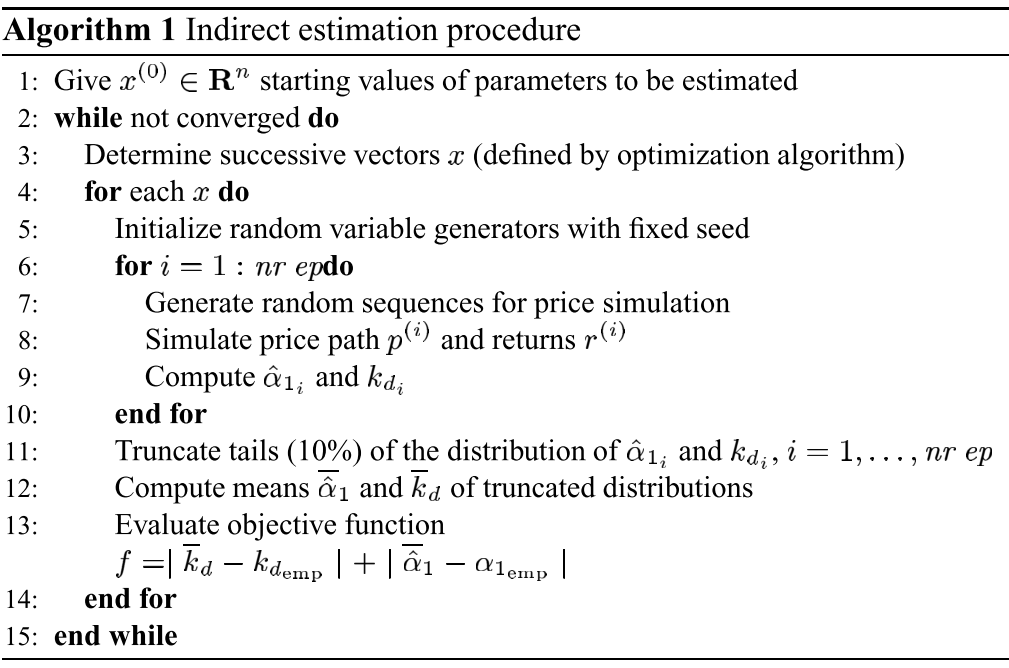
\includegraphics[scale=.25]{figures/gilli_2001_algorithm.png}
		\caption{The \citet{gilli2001estimation} algorithm for indirect inference of the two parameters $(\varepsilon, \delta)$.}
	\end{figure}
\end{frame}


\begin{frame}[c]\frametitle{Surface plot}
	\begin{figure} \centering
		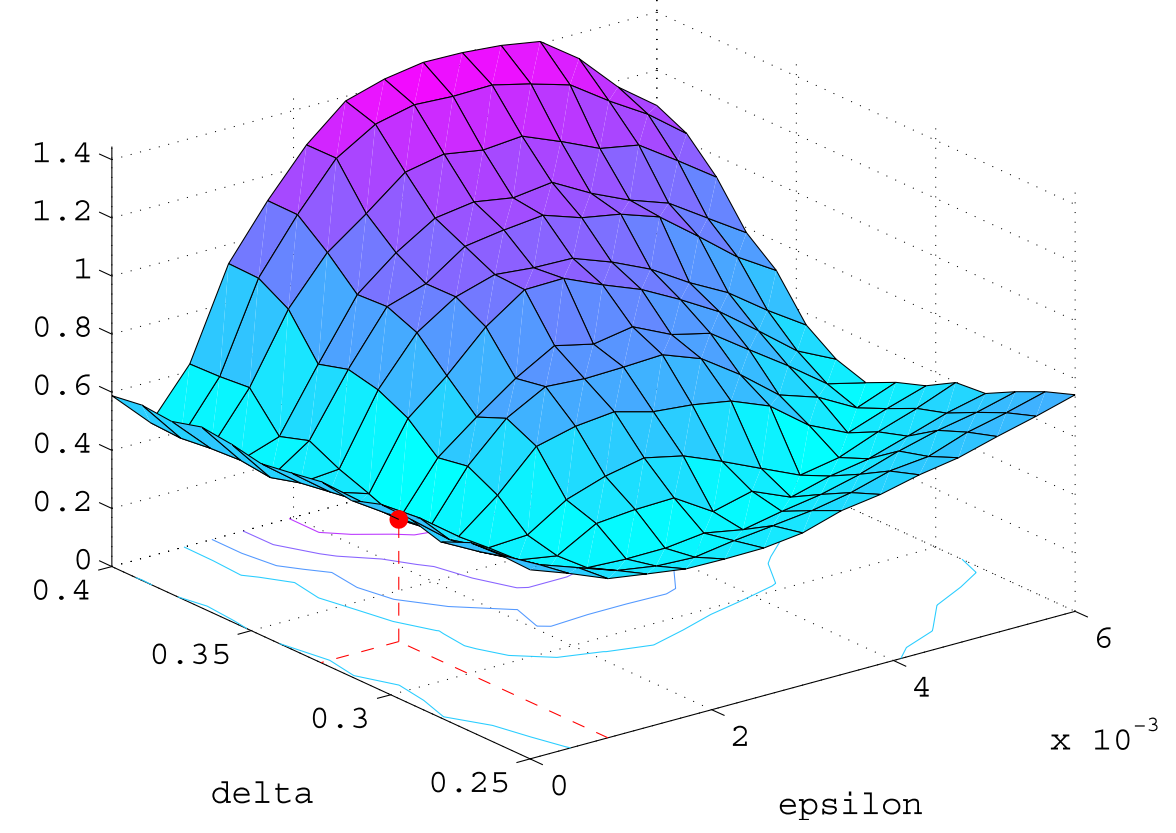
\includegraphics[scale=.25]{figures/gilli_2001_surface.png}
		\caption{The \citet{gilli2001estimation} surface plot of $f$ over the $(\varepsilon, \delta)$ space.}
	\end{figure}
\end{frame}


\begin{frame}[c]\frametitle{What does this exercise tell us?}
    Optimal estimate is $(\varepsilon^{*}, \delta^{*}) = (0.00086,0.325)$. \bigskip

    \alert{\textbf{Economic implications}}
    \\ In the \citet{kirman1991epidemics} model the dynamic converges to a coexistence of fundamentalist and chartist agents if $\varepsilon < (1-\delta)(N-1)$.\footnote{Where $N=100$ is the number of traders.} \bigskip

    Hence, bringing the data to the model might suggest that the DGP of the empirical observation is better approximated by a model where the switching between the fundamentalist and chartist trading strategies matters. \bigskip

    The estimation seems to conclude that the relative fractions of fundamentalist and chartist traders aren't constant over time.
\end{frame}


\begin{frame}[c]\frametitle{Limitations}
    \citet{gilli2001estimation} recognize that:
    \begin{itemize}
    	\item the two moments do not provide a sufficient description of the exchange rate dynamics (hence this estimation in hardly a test on the theory of exchange rate determination);
    	\item further features (additional moments) shall be taken into account to better discriminate between different models;
    	\item including other moments would however require more computational power (which was limited in 2001, but is less of a problem today for simple small-scale models).
    \end{itemize}

    In addition: 
    \begin{itemize}
    	\item the truncation of the $10\%$ tails can be debated;
    	\item the distance $f$ is additive with same weights of the two objective. One can think of many possible functional forms or at different weights combinations;
    	\item there are other parameters which have not been estimated. What about, for example, the effects of the parameter $\nu$?
    \end{itemize}
\end{frame}


\begin{frame}[c]\frametitle{The heritage of \citet{gilli2001estimation}}
    \citet{gilli2001estimation} set the ground for the development of the literature in the estimation of ACE models. \bigskip

    The main algorithmic procedure adopted has been extensively used with some variations and improvements:
    \begin{itemize}
    	\item \citet{alfarano2005estimation}: simpler model with an analytical closed form solution for the distribution of returns and, therefore, direct and parametric (rather than indirect) estimation of the parameters; \smallskip
    	\item \citet{franke2012contest}: two models (with at most 8 parameters) estimated with respect to 9 selected moments by minimization of a weighted quadratic loss function; introduction of the \emph{moment coverage ratio (MCR)} concept; \smallskip
    	\item \citet{kukacka2017estimation}: estimation of the \citet{brock1998heterogeneous} model by means of non-parametric simulated maximum likelihood estimation (NPSMLE).
    \end{itemize}
\end{frame}


\subsection{Grazzini and Richiardi (2017)}


\begin{frame}[c]\frametitle{\citet{grazzini2017bayesian}}
	Introduction of Bayesian techniques to estimate ABM with applications to the \citet{cliff1997minimal} model as well as to a New Keynesian model (mid-scale). \bigskip

	\alert{\textbf{Advantages}}
	\begin{itemize}
		\item does not require pre-selected moments to evaluate the model quality;
		\item incorporates prior knowledge and copes better with uncertainty;
		\item uses all the information coming from the data. %(i.e. the whole distribution).
	\end{itemize}

	\alert{\textbf{Drawbacks}}
	\begin{itemize}
		\item can mask identification issues by adding curvature to possibly flat likelihood functions;
		\item it is computationally demanding since the likelihood estimation might require as much time as the simulation of the model;
		\item when approximating the likelihood, the extent of the first advantage is reduced.
	\end{itemize}
\end{frame}


\begin{frame}[c]\frametitle{Bayes theorem}
	Bayes theorem applied to the real data, as possibly derived by the model as a DGP writes:
    \begin{equation} \label{eq:bayes}
    	p(\theta | y) \propto \mathcal{L}(\theta; y) \cdot p(\theta)
    	% \propto p(y | \theta) \cdot p(\theta)
    \end{equation}
	where:
	\begin{itemize}
		\item $p(\theta | y)$ is the \emph{posterior} distribution of the parameters $\theta$;
		\item $\mathcal{L}(\theta; y) = p(y | \theta)$ is the likelihood of observing the data $Y^{R}$ conditional on the simulation parameter vector $\theta$;
		\item $p(\theta)$ is the \emph{prior} distribution of the parameters $\theta$;
	\end{itemize} \bigskip

	\alert{\textbf{Major difference with SMD}}
	\\ The outcome of the estimation is a multivariate distribution (univariate over each of the components of the parameter vector $\theta$) and not a single point estimate.
\end{frame}


\begin{frame}[c]\frametitle{Estimating the likelihood}
    The central issue of the Bayesian approach is the estimation of the likelihood function $\mathcal{L}(\theta; y)$. \bigskip

    \alert{\textbf{Non-parametric estimation} (slower)}
    \begin{equation*}
    	\mathcal{L}(\theta; y) = \prod_{t=1}^{T} g(y_{t}^{R} | \theta)
    \end{equation*}
    and the estimate $\hat{g}$ is performed trough Kernel density estimation (KDE) using the simulated data after the statistical equilibrium has been reached.\footnote{Ergodicity and stationarity of the model are required.} \bigskip

    \alert{\textbf{Parametric estimation} (faster)}
    \begin{equation*}
    	y_{t} = g^{*}(\theta) + \varepsilon_{t}
    \end{equation*}
    The functional form of $g^{*}$ is here assumed to have some convenient form (e.g. Gaussian) but if the assumption is wrong, estimation biases are likely to arise. \bigskip
\end{frame}


\begin{frame}[c]\frametitle{Iteration over $\theta$}
	Once the likelihood is estimated, the application of Bayes theorem in equation~\ref{eq:bayes} allows one to obtain a density for the posterior at one given value of $\theta$. \bigskip

	But to recover the whole posterior distribution one shall sample for different $\theta \in \Theta$ (as in the standard indirect inference approach) and simulate the models at many different values.\bigskip

	Thus, if $\theta$ has length $K$ and each element $\theta_{k}$ is sampled at $J$ different values, we need to estimate the likelihood a number of times equal to $N_{\mathcal{L}} = J^K$. \bigskip

	All in all, the model requires $N = N_{\mathcal{L}} \cdot M$ independent simulations.
\end{frame}


% \begin{frame}[c]\frametitle{Application to the \citet{cliff1997minimal} model}
%     The \citet{cliff1997minimal} model embeds N agents that trade on the order-book:
%     \begin{itemize}
%     	\item limit price in $t$: $p_{i,t} = \nu_{i} (1 + \mu_{i,t})$;
%     	\item adjustment in $t$: $\Delta_{i,t} = \beta (\tau_{i,t} - p_{i,t})$;
%     	\item limit price in $t+1$: $p_{i,t+1} = p_{i,t} + \Delta_{i,t}$;
%     	\item profit margin in $t+1$: $\mu_{i,t+1} = \frac{p_{i,t+1}}{\nu_{i}} - 1$.
%     \end{itemize} \bigskip

%     Pseudo-true value: $\beta = 0.55$ with 11 agents. \bigskip
% \end{frame}

\begin{frame}[c]\frametitle{Estimation with parametric and non-parametric strategies}
	\begin{figure} \centering
		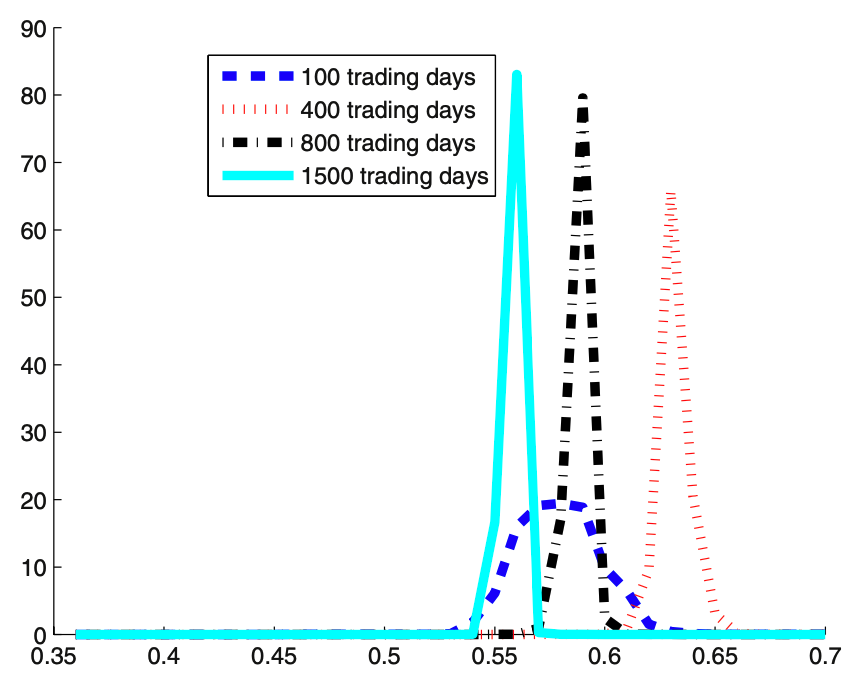
\includegraphics[scale=.11]{figures/grazzini_2017_gaussian.png} ~
		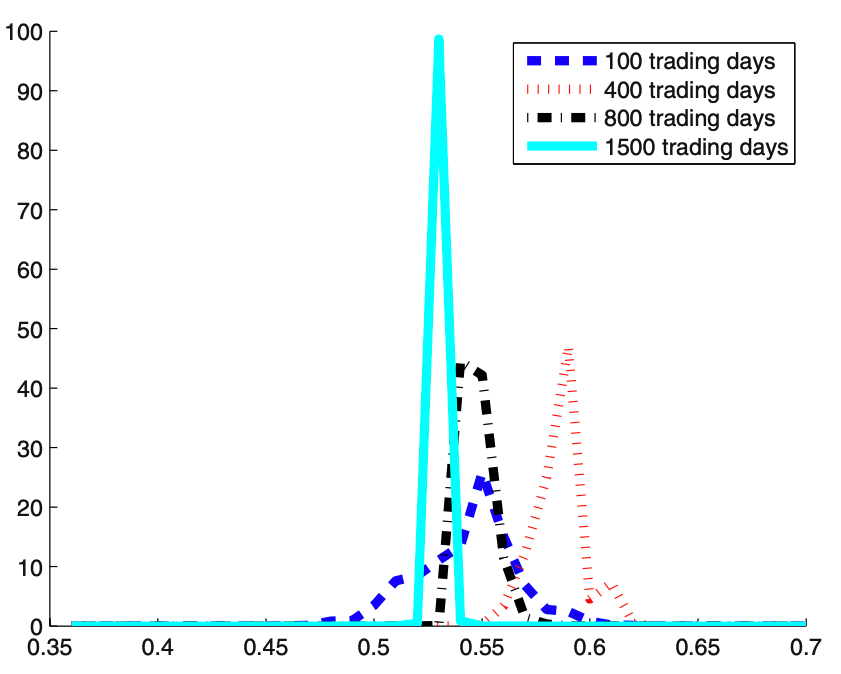
\includegraphics[scale=.11]{figures/grazzini_2017_grid.png} ~
		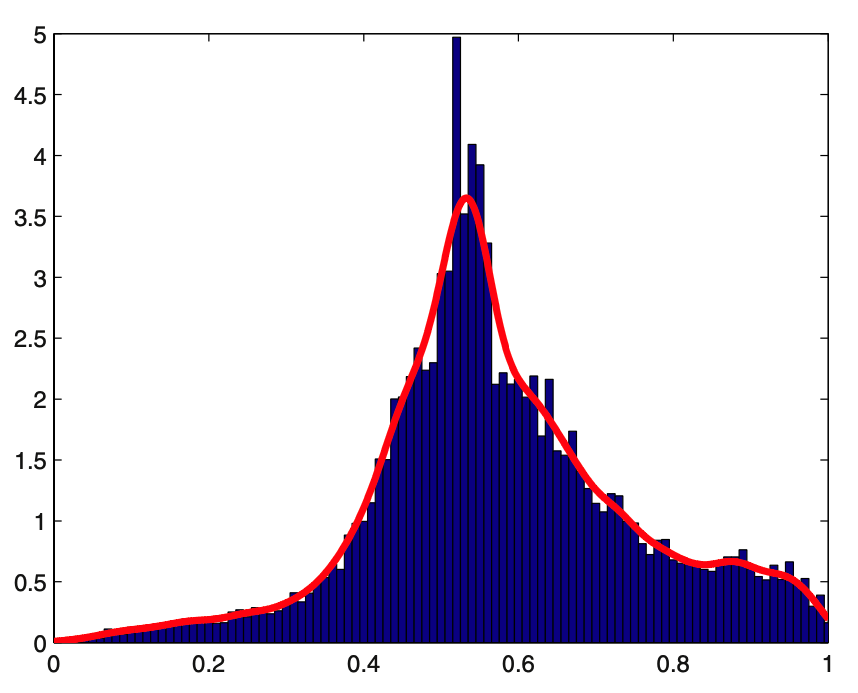
\includegraphics[scale=.11]{figures/grazzini_2017_mcmc.png}
		\caption{Posterior distribution of the parameter $\beta$ under grid search and Gaussian parametric estimation, grid search with KDE and MCMC search with KDE.}
	\end{figure} \vspace*{-.5cm}

	\alert{\textbf{Results}}
	\begin{itemize}
		\item Parametric Gaussian: highest precision;
		\item KDE with grid search: quite precise but biased;
		\item KDE with MCMC search: quite imprecise.
	\end{itemize} \bigskip
\end{frame}


\begin{frame}[c]\frametitle{Estimation with the ABC strategy}
	\begin{figure} \centering
		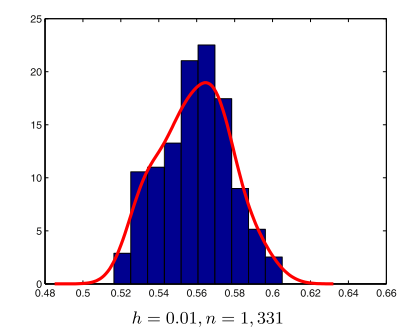
\includegraphics[scale=.26]{figures/grazzini_2017_abc1.png} ~
		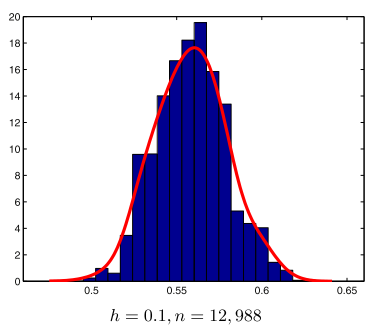
\includegraphics[scale=.26]{figures/grazzini_2017_abc2.png} ~
		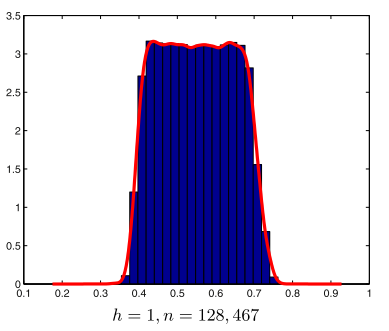
\includegraphics[scale=.26]{figures/grazzini_2017_abc3.png}
		\caption{Posterior distribution of the parameter $\beta$ under Approximate Bayesian Computation algorithm, with KDE estimated at different bin-width values.}
	\end{figure} \vspace*{-.5cm}

	\alert{\textbf{Result}}
	\begin{itemize}
		\item Approximate Bayesian Computation as good as the parametric one in the best case;
		\item but the results are sensitive to the KDE bin-width choice;
		\item in particular there is a trade-off between bin-width and estimation uncertainty.
	\end{itemize} \bigskip
\end{frame}


% estimation in high-dimensions ------------
\section{Estimation of large-scale ABM}
\label{sec:largescale_abm}


% \begin{frame}[c]\frametitle{Estimation or fine tuning?}
% 	\begin{figure} \centering
% 		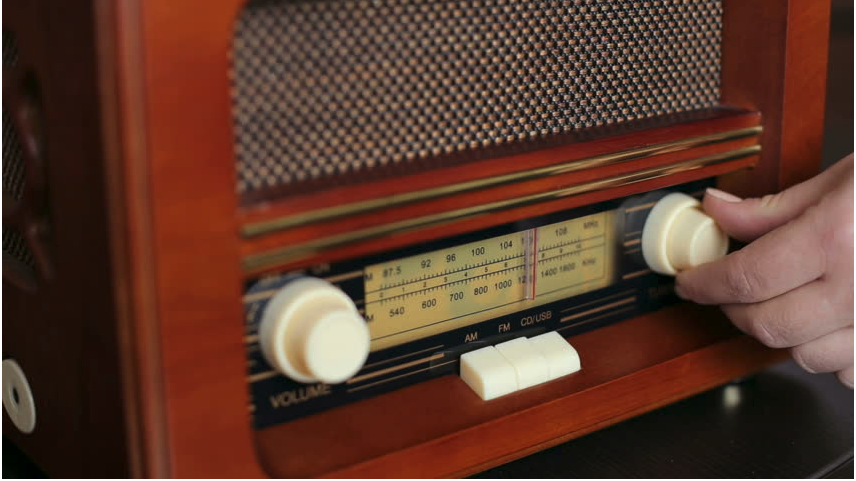
\includegraphics[scale=.36]{figures/example_tuning.png}
% 	\end{figure}
% \end{frame}


\begin{frame}[c]\frametitle{Estimation via method of simulated moments}
	To our knowledge, only two mid-scale models estimated via MSM:
	\begin{itemize}
		\item \citet{bianchi2007calibrating}: macroeconomic model;
		\item \citet{guerini2020governance}: industry dynamics model.
	\end{itemize}
	The biggest issue remains the computational burden, which is accompanied by the \emph{curse of dimensionality} \citep{de2005book}. \bigskip

	\begin{alertblock}{Example: Calibrating the \citet{dosi2015fiscal} model}
		\begin{itemize}
			\item number of parameters: $K = 31$;
			\item number of Monte Carlo: $M = 100$;
			\item grid search of equispaced points for each parameter: $J = 20$;
			\item simulation time of a run: $T = 60s$.
		\end{itemize} \smallskip
		Required independent simulations: $M \cdot J^{K} = 2.15 \cdot 10^{42}$ runs; \\
		Required computational time: $T \cdot M \cdot J^{K} = 3.58 \cdot 10^{40}$ hours.	
	\end{alertblock}
\end{frame}


\subsection{Lamperti, Sani, Roventini (2018)}


\begin{frame}[c]\frametitle{Meta-models}
	At this stage, is clear that the two most computationally intensive tasks for estimating an ABM are:
	\begin{itemize}
		\item running the model;
		\item computing the likelihood / evaluating the distance.
	\end{itemize} \medskip

	One approach to fasten the times of evaluation is that of replacing the model with a \emph{surrogate} (a.k.a. meta-model) and evaluating its quality. \medskip

	\alert{\textbf{What is a meta-model?}}
	\\ Is a model/function which approximates the relation between the inputs of the complete ABM with its output. Allows one to evaluate the variation in the model outcomes over the parameter space without simulating the model. \medskip

	Two possible approaches:
	\begin{itemize}
		\item parametric \citep[see][]{salle2014kriging,dosi2018sensitivity}
		\item non-parametric \citep[see][]{lamperti2018surrogates}
	\end{itemize}
\end{frame}


\begin{frame}[c]\frametitle{Procedure}
To carry out the exercise and evaluate the performance of the model the following procedure is followed:
	\begin{enumerate}
		\item draw a relatively large set of points using any standard sampling routine (e.g. NHLH) to proxy the whole parameter space;
		\item employ a small random subset of these points, simulate the ABM and classify them (positive or negative label) to learn a surrogate model (i.e. a classifier system);
		\item learn the surrogate model and use it to predict the probability of all the other non-classified points to be positively labelled;
		\item select a small random subset of the points classified by the surrogate (with high probabilities of being positive) and evaluate them against the ABM output;
		\item repeat steps 2 to 4 until a satisfactory level of performance is achieved or until a predefined number of iterations (a.k.a. \emph{budget}) is completed.
	\end{enumerate}
\end{frame}


\begin{frame}[c]\frametitle{Crucial Steps}
	\alert{\textbf{Definition of a positive calibration}}
	\\ A positive calibration is a parameter vector $\theta \in \Theta$ such that the model's outcome satisfies a predefined calibration criterion. \bigskip

	\alert{\textbf{Selection of the learning algorithm}}
	\\ Usage of XGBoost (a gradient boosting algorithm) that produces a statistical model that classifies/labels the sampled points. \bigskip

	\alert{\textbf{Surrogate performance}}
	\\ Binary case: $\underset{\mathcal{F}}{argmax} ~ F_{1} =\frac{2 \cdot \text{true positives}(\theta; \mathcal{F})}{2 \cdot \text{true positives}(\theta; \mathcal{F}) + \text{false positives}(\theta; \mathcal{F}) + \text{false negatives}(\theta; \mathcal{F})}$ 
	\\ Real-valued case: $\underset{\mathcal{F}}{argmin} ~ MSE = \frac{\sum_{i=1}^{N}(\hat{y}_{i}(\theta; \mathcal{F}) - y_{i}(\theta))^2}{N}$ \bigskip

	\alert{\textbf{Out-of-sample evaluation}}
	\\ Use of the true positive rate $TPR = \frac{\text{number of correctly predicted positives}}{\text{number of positives in the pool}}$
\end{frame}


\begin{frame}[c]\frametitle{Application to the \citet{dosi2003island} \emph{island model}}
	\alert{\textbf{Surrogate model selection criteria}}
	\begin{itemize}
		\item average GDP growth above 2\%;
		\item output growth rates with AEP distribution with $b \leq 1$.
		\item no exercise with real data; the aim of the paper is that of evaluating the goodness of fit of the surrogate (not of the \citet{dosi2003island} \emph{island model}).
	\end{itemize}

	\alert{\textbf{Results}}
	\begin{itemize}
		\item surrogate modelling is 3750 times faster than the fully-fledge \emph{island model};
		\item with a sufficient \emph{budget}, the surrogate model can out-of-sample correctly classify 90\% of the points.
	\end{itemize}
\end{frame}


\begin{frame}[c]\frametitle{The meta-model as a descriptive device}
    \begin{figure} \centering
    	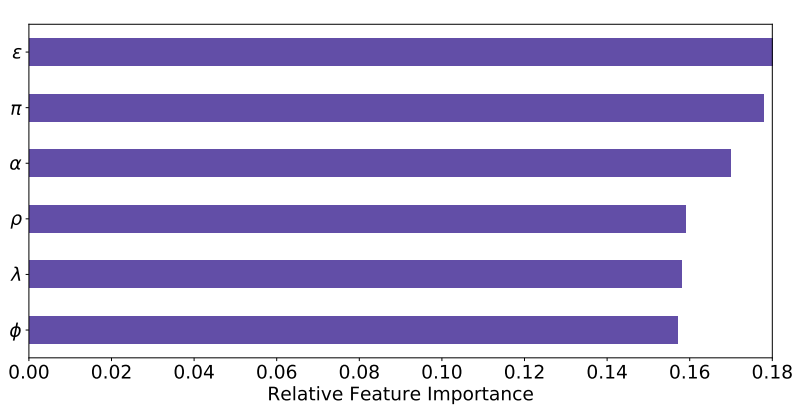
\includegraphics[scale=.25]{figures/lamperti_2018_featureimportance.png}
    	\caption{Importance of each parameter in shaping behaviour of the Islands model according to the specified criteria.}
    \end{figure}

    \alert{\textbf{Results}}
    \begin{itemize}
    	\item The meta-model can be used to decompose the variance of the explained objective as a function of to the parameters;
    	\item here all the parameters are almost equally important;
    	\item the parameter $\varepsilon$ is slightly more relevant, meaning that small modifications of it can affect the calibration exercise to a larger extent.
    \end{itemize}
\end{frame}


\begin{frame}[c]\frametitle{Assessment of the strategy}
    \alert{\textbf{Advantages}}
    \begin{itemize}
    	\item fast due to the fact that one doesn't need to simulate the ABM many times;
		\item when the response surface to a variation in the parameters is very rugged, the surrogate is able to capture them;
		\item allows one also to assess the parameters importance and to avoid modifying parameters that do not affect the model's outcome.
    \end{itemize} \bigskip
    
    \alert{\textbf{Drawbacks}}
    \begin{itemize}
    	\item the meta-model might not be a sufficient good representation of the ABM;
    	\item when the response surface to a variation in the parameters is smooth, parametric alternatives can be more efficient;
    	\item the surrogate is difficult to interpret: for policy analysis one needs to resort to simulation of the ABM.
    \end{itemize}
\end{frame}


% new measures -------------------------------
\section{New Distances and Objective Functions}
\label{sec:new_objectives}


\begin{frame}[c]\frametitle{New metrics for validation of ACE model}
	In the recent years a series of new distances to evaluate the performance of an ACE model against real data have been developed. \bigskip

	Among them:
	\begin{itemize}
		\item \citet{marks2013validation};
		\item \citet{barde2017practical,barde2020comparison}
		\item \citet{lamperti2018gsl}
		\item \citet{guerini2017validation}
	\end{itemize} \bigskip

	Current research is in the attempt of using these distances as minimization criteria for medium- and large-scale models in order to estimate them over a large number of parameters.
\end{frame}

\begin{frame}[c]\frametitle{Are real and simulated data similar?}
	\begin{figure} \centering
	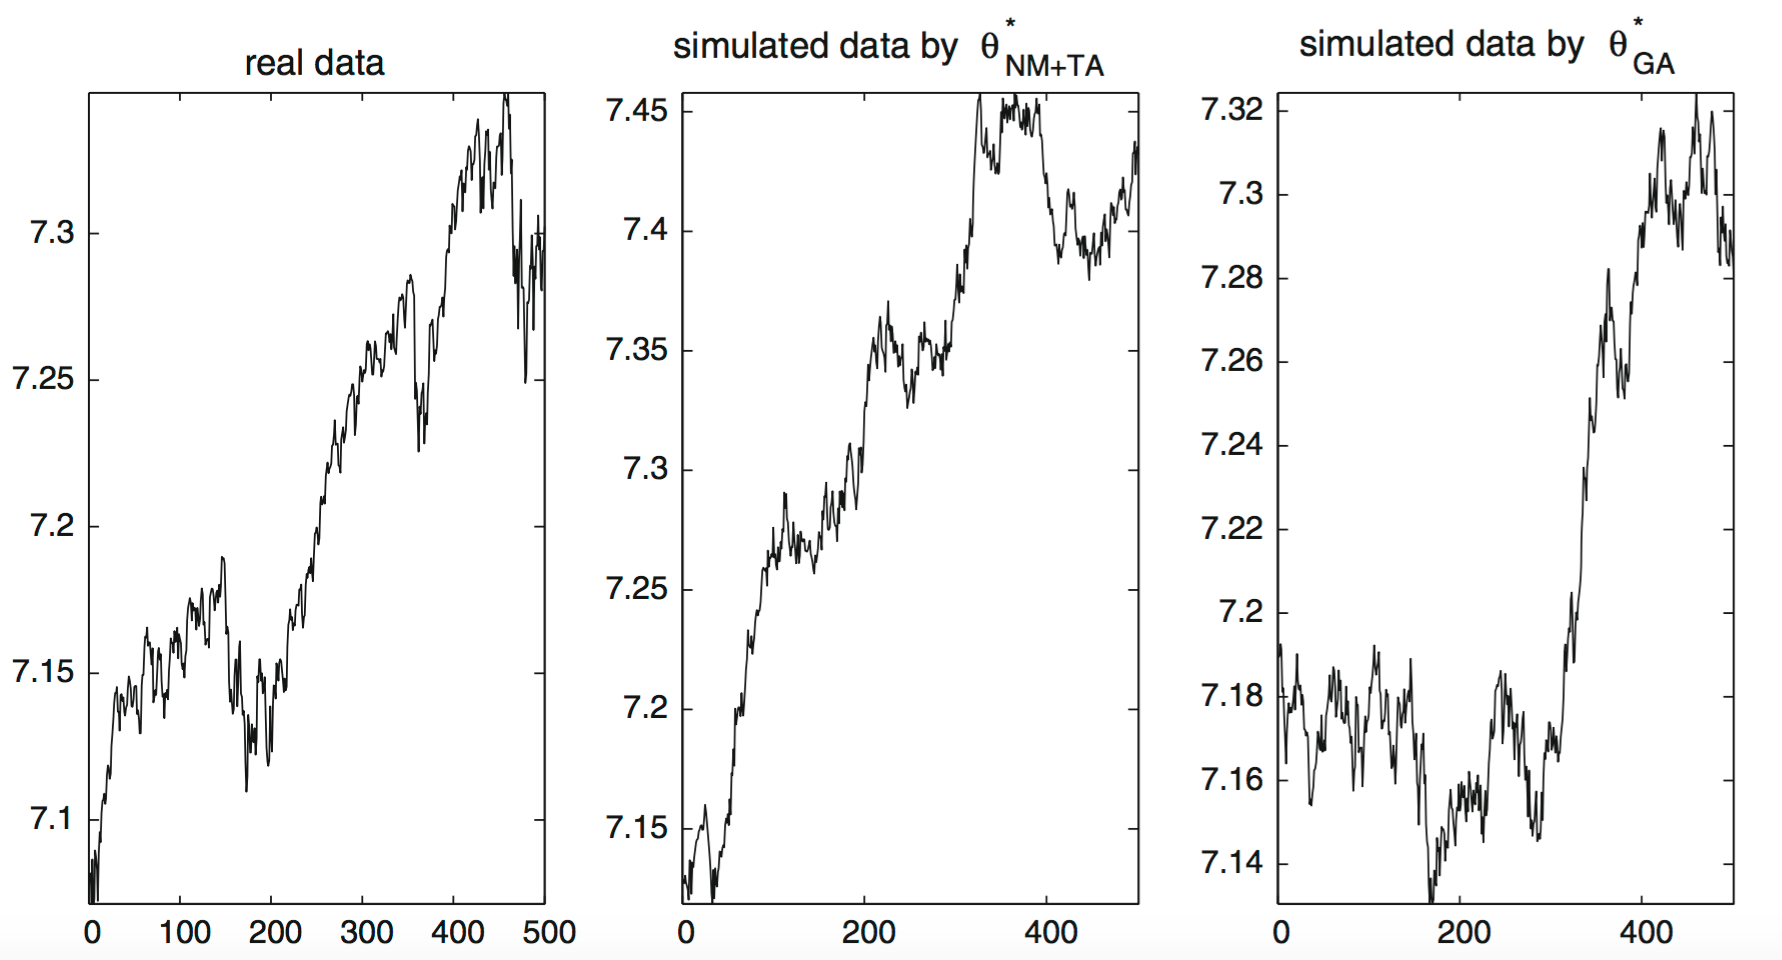
\includegraphics[scale=0.3]{figures/fabbretti_2003_timeseries.png}\\
	Source: \cite{fabretti2013problem}
	\end{figure}
\end{frame}

\begin{frame}[c]\frametitle{The KL divergence}
	\begin{itemize}
		\item Estimate the conditional distribution of patterns emerging from real and simulated  data
		\item Compare the two distributions
	\end{itemize}

	A well known measure of the distance between distributions, with well known theoretical properties, is the Kullback-Leibler divergence:
	\begin{equation}
		D_{KL}(\textbf{p}||\textbf{q})=\sum_{s \in \textit{S} }p(s)\log\left(\frac{p(s)}{q(s)}\right),
	\end{equation} 

	The KL divergence measures the information loss when assuming that a distribution is $q$ while the true one is $p$.
\end{frame}

\begin{frame}[c]\frametitle{Alternative distance measures}
	A \alert{\textbf{set of criteria}} has been developed to capture the distance between real and simulated data:
	\begin{itemize}
		\item the State Similarity Measure \citep[SSM --][]{marks2013validation};
		\item the Markov Information Criterion \citep[MIC --][]{barde2017practical, barde2020comparison};
		\item the Generalized Subtracted L-divergence \citep[GSL-div --][]{lamperti2018gsl, lamperti2018empirical}.
	\end{itemize}
	\smallskip
	
	\alert{\textbf{Similarities and trade-offs}:}
	\begin{itemize}
		\item they are all built upon information theory concepts;
		\item But they capture slightly different features;
		\item And they have different computational burdens ($\text{time}_{\text{MIC}}>\text{time}_{\text{GSL}}>\text{time}_{\text{SSM}}$)
	\end{itemize}
\end{frame}

\begin{frame}[c]\frametitle{The GSL-div by \citet{lamperti2018gsl}}

	It measures the \alert{\textbf{distance between the regularity of behaviours}} observed in the empirical data and that of simulated data. \bigskip

	It is constructed through a \alert{\textbf{simple algorithm}}
	\begin{enumerate}
		\item Time series are symbolized into b symbols
		\item Sequences of symbols (words) are observed using multiple rolling window of maximal length L
		\item Distributions are compared using a well known information theoretic divergence measure (L-div)
		\item They are iteratively aggregated using weights that penalize short windows
	\end{enumerate}

	Parameters $b$ and $L$ need to be fine-tuned.
\end{frame}

\begin{frame}[c]\frametitle{Symbolization}
    \begin{figure}[!ht] \centering
    	\caption*{ }
        \begin{subfigure}[b]{0.5\textwidth} \centering
            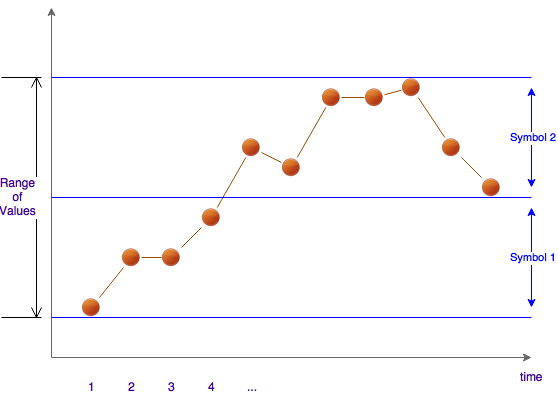
\includegraphics[width=0.9\textwidth]{figures/lamperti_2018_simb1.png}
            \caption{$b\, \text{(precision of symbolization)} =2$}
        \end{subfigure}%
        ~
        \begin{subfigure}[b]{0.5\textwidth} \centering
			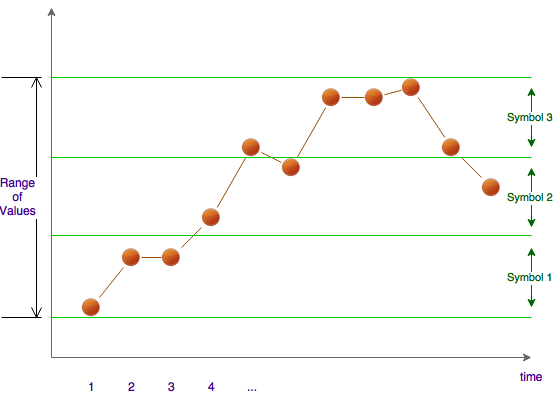
\includegraphics[width=0.9\textwidth]{figures/lamperti_2018_simb2.png}
            \caption{$b\, \text{(precision of symbolization)} =3$}
        \end{subfigure}
	\end{figure}
\end{frame}

\begin{frame}[c]\frametitle{Matching Causality by \citet{guerini2017validation}}
	Is the mere replication of stylized facts or distribution a hard test for evaluating the model quality? If the answer is no, then one shall focus on \alert{\textbf{causal relationships}}. \bigskip
	
	The intuition is that models with different causal structures, might generate equivalent statistical properties (i.e. the same stylized facts).

	How to discriminate between them?
	\begin{itemize}
		\item estimate the causal structures emerging from real-word data and model-generated data;
		\item compare them in a meaningful way.
	\end{itemize} 
\end{frame}

\begin{frame}[c]\frametitle{The procedure}
	\medskip
    \begin{minipage}{0.45\textwidth}
	    \begin{figure}\centering
	    	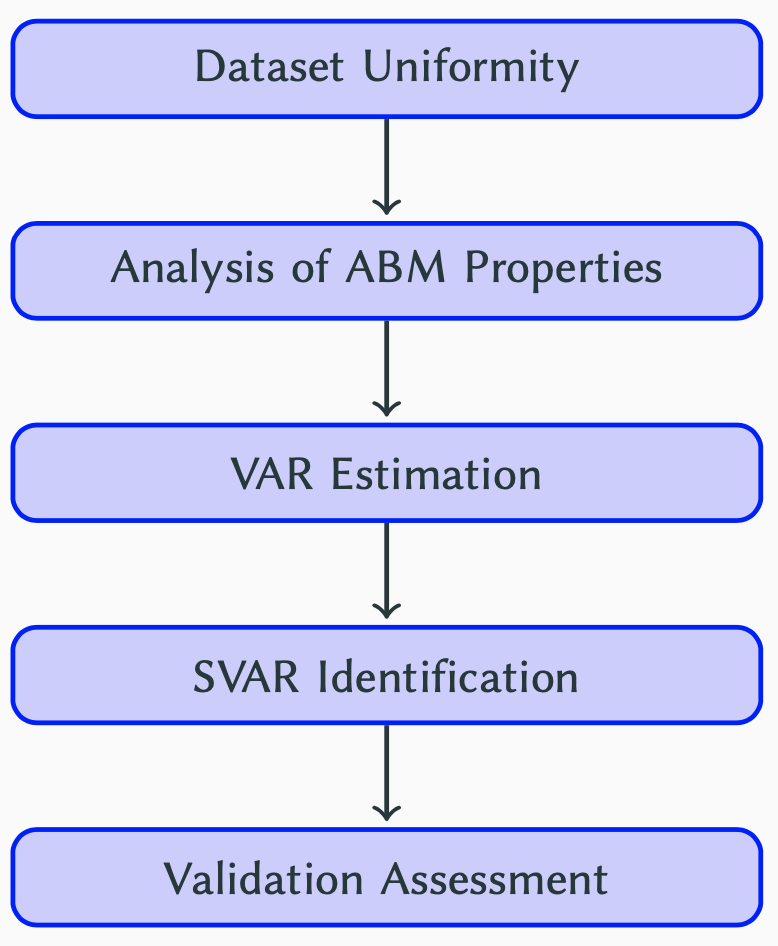
\includegraphics[scale=.35]{figures/guerini_2017_procedure.png}
	    \end{figure}
    \end{minipage}~
    \begin{minipage}{0.5\textwidth}
    	\alert{\textbf{Ergodicity and stationarity}} can be tested by batteries of Kolmogorov-Smirnov tests. \medskip

    	The SVAR identification can be done by modern causal search algorithms with relatively mild assumptions, without imposing \alert{\textbf{a-priori restriction}}. \medskip

    	The \alert{\textbf{similarity}} is computed using signs and magnitudes of the causal relationships estimated on the real and on the simulated data.
    \end{minipage} \medskip

    Application has been done at the moment on the \citet{dosi2015fiscal} model. \smallskip

    Currently on-going: a comparison of \citet{grazzini2017bayesian} and \citet{guerini2017validation} on the \citet{delligatti2015jeic} model.
\end{frame}

% new measures -------------------------------
\section{Conclusions}
\label{sec:conclusion}

\begin{frame}[c]\frametitle{Overall Evaluation}
	After almost 20 years from the \cite{gilli2001estimation} seminal contribution:
	\begin{itemize}
		\item computational power has hugely increased expanding the possibilities for estimation and calibration of ACE models;
		\item many alternative nuances of the estimation method are now available, but their applications by ACE modellers is still scant.
	\end{itemize} \medskip

	\alert{\textbf{The quest for the \emph{optimal estimation strategy}?}}
	\\ Probably not, as all methods have advantages and drawbacks. \medskip

	Future research will likely aim at:
	\begin{itemize}
		\item specifying the statistical properties of the different estimators as well as the conditions for their usage to better define the applicability domains of the different methods;
		\item writing a broad open-source software embedding most of the methodologies to allow ABM economists and policy-makers to easily implement them.
	\end{itemize}
\end{frame}

\begin{frame}[c]\frametitle{A Validation Cookbook for AB Modellers} \small
	Ideal procedure for \textit{descriptive models}:
	\begin{enumerate}
		\item \alert{\textbf{input validation}:} build the model by grounding behavioural rules and interaction mechanisms on the empirical or experimental literature 
		\item \alert{\textbf{estimation}:} decide the real-world data, the moments to match and estimate the model with the preferred method
		\item \alert{\textbf{estimation robustness}:} run Monte Carlo simulations and check if the model dynamics resembles the real world one according to some distance measure
		\item \alert{\textbf{stylized facts replication}:} check which stylized facts the model can replicate (in addition to the ones used for the estimation)
		\item \alert{\textbf{causal structure validation}:} check if the model causal structure resembles the one that emerges from the real data (if the model has policy implications, this is particularly relevant)
		\item \alert{\textbf{sensitivity analysis}:} run local sensitivity analysis or use a surrogate to globally explore the parameter space
		\item \alert{\textbf{policy analysis}:} run policy exercises and compare results to the baseline parametrization
	\end{enumerate}
\end{frame}


% standout ---------------------------------
\begin{frame}[standout]
	Thanks for the attention.
\end{frame}


% bibliography -----------------------------
\begin{frame}[c, allowframebreaks]\frametitle{References}
	\vspace{-1.2cm}
 	\footnotesize
	\bibliographystyle{chicago}
	\bibliography{biblio} 
\end{frame}


\end{document}

